\chapter{Limitations}
\label{sec:limitation}
The results in Chapter \ref{sec:evaluation} showed that the measured heart rate could be input to the smartwatch with small errors in most cases. This chapter discusses the limitations of the proposed method in terms of other pulse-wave-related indices and the pulse waveform.\par

For comparison, I acquired real raw PPG data from my left index finger and raw PPG data generated by display D with a 2-mm acrylic plate. Figure \ref{fig:raw_data_acquisition} illustrates the environment during this raw pulse data acquisition. Numerical pulse data was collected at a sampling rate of 106 Hz for 60 s by using an Arduino Uno R3 and a PPG sensor\footnote{\url{https://www.pulsesensor.com}}. The Arduino used here was different from the one used to control the display.

\begin{figure}[!t]
  \centering
  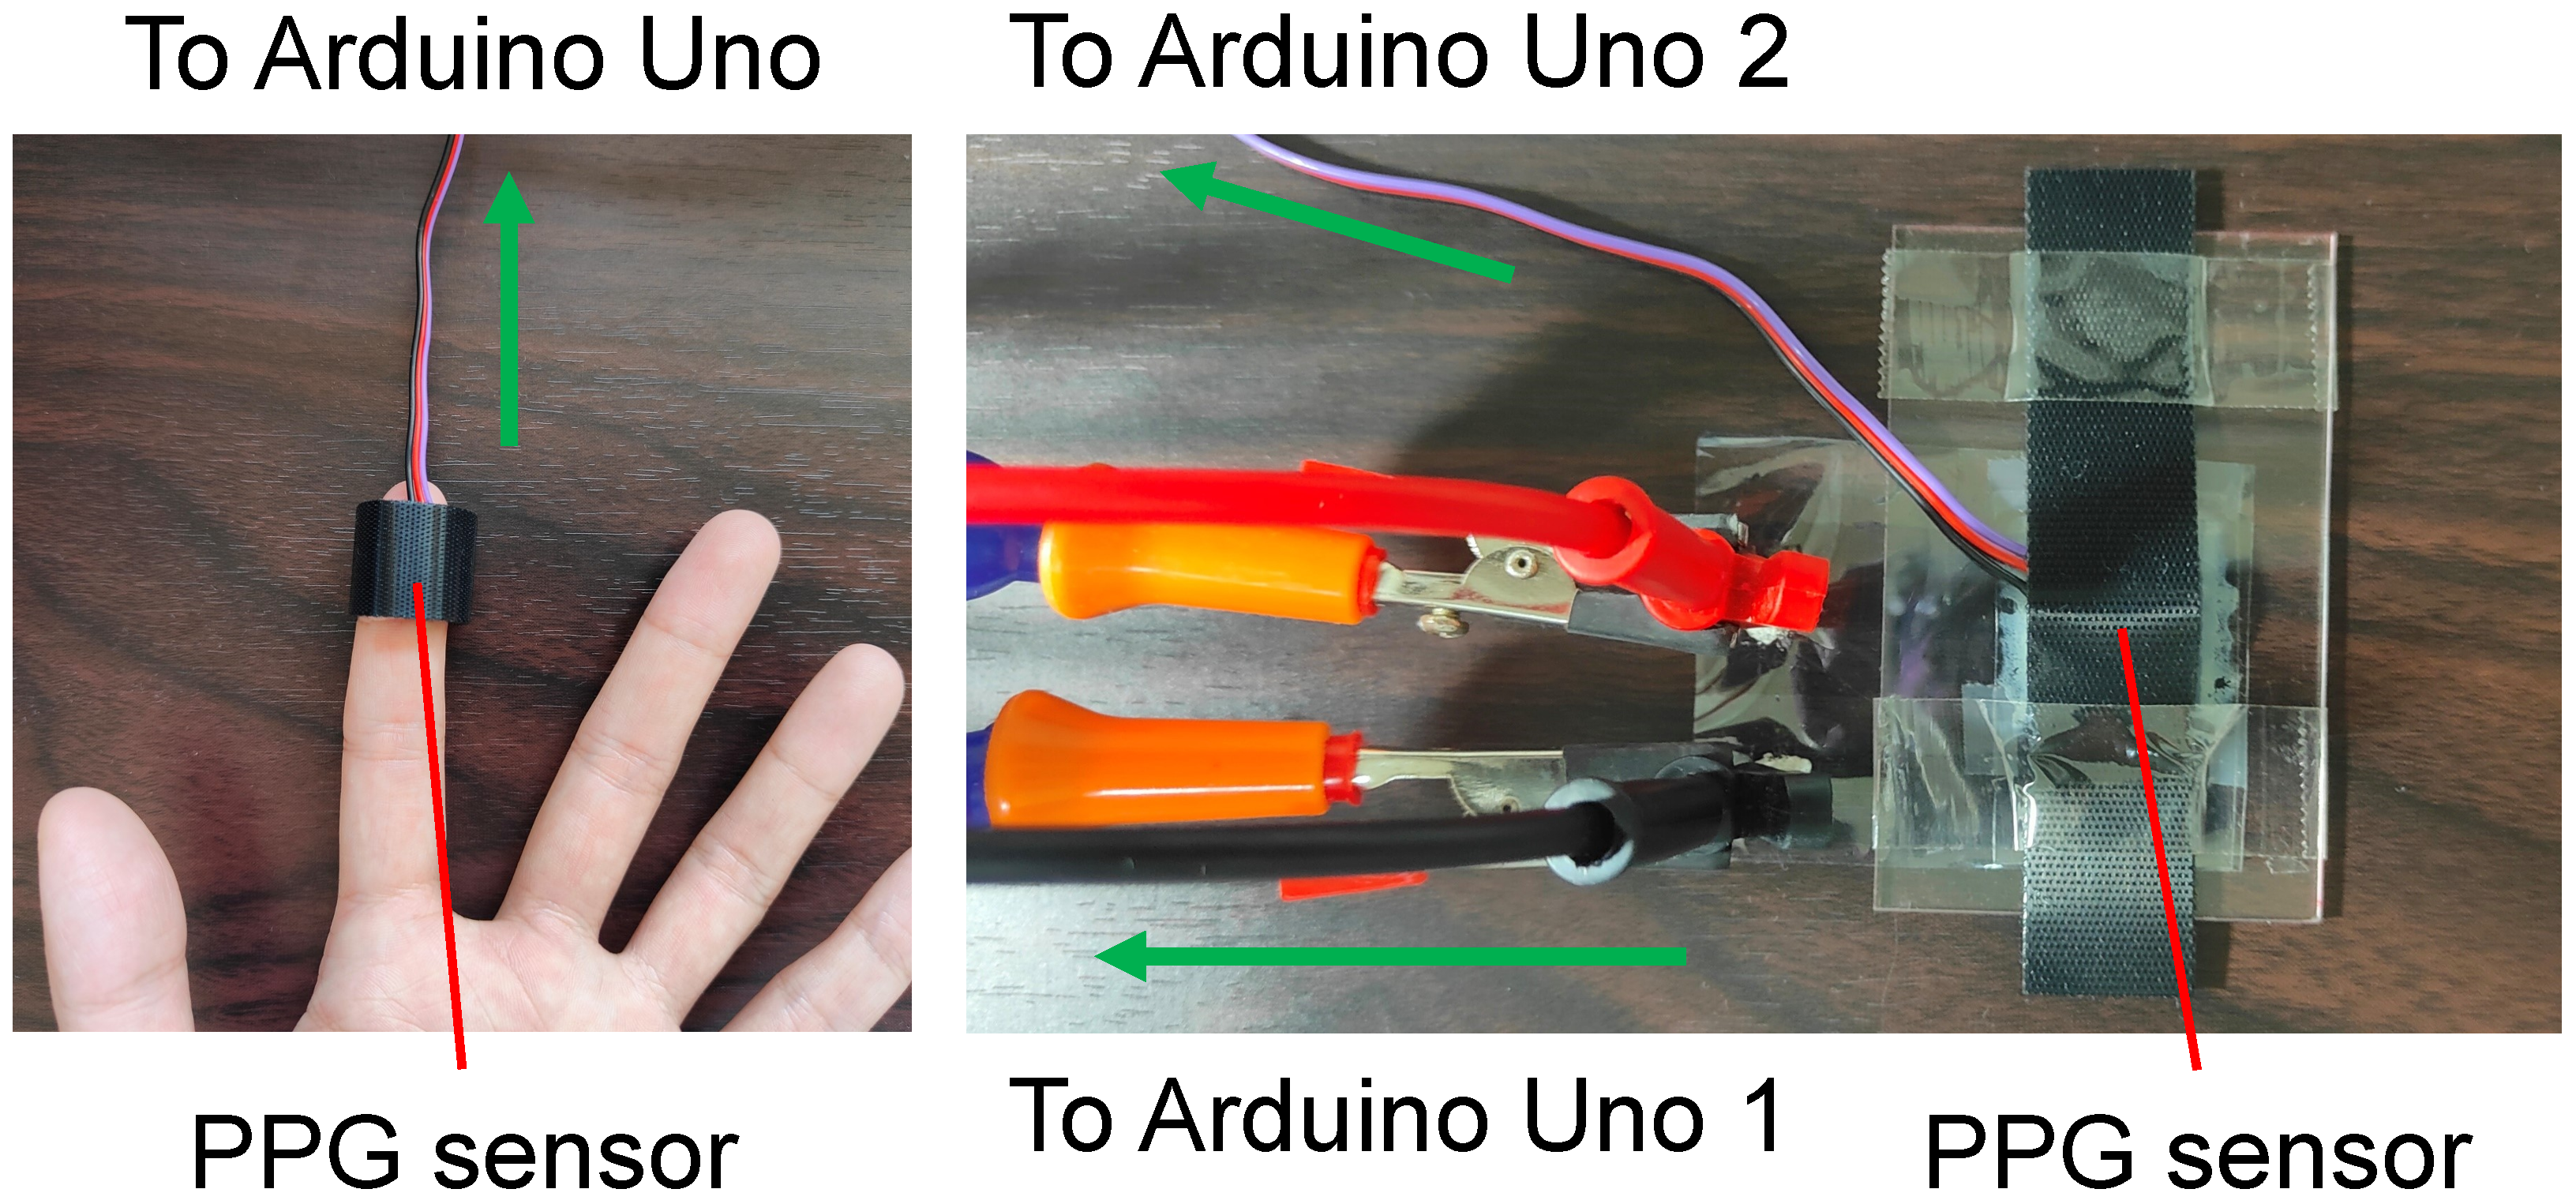
\includegraphics[width=1\linewidth]{figures/raw_data_acquisition.eps}
  \caption{Environment during raw pulse data acquisition.}
  \label{fig:raw_data_acquisition}
\end{figure}


% 5.1
\section{Pulse Wave Status Indicators}
The raw PPG data was analyzed using Kubios HRV Premium (ver. 3.5.0)\footnote{\url{https://www.kubios.com/hrv-premium}}, a fully featured heart rate variability (HRV) analysis software package. Figure \ref{fig:rr_wave} shows the resulting RR time series data, Table \ref{tab:report_real} lists the analysis results for the real PPG data, and Table \ref{tab:report_generated} lists the results for the generated PPG data. The values in these analysis results were calculated from the RR time series data. The target heart rate at the time of pulse wave generation was set to 68 bpm, which was the mean heart rate (HR) of the real pulse wave obtained from the finger.\par

The results showed that the generated pulse wave was at 68 bpm for both the minimum HR and the maximum HR. They also showed that the target heart rate could be input to the PPG sensor in a stable manner, as in the main experiment described in Chapter \ref{sec:evaluation}. As for the RR interval, it is regular under normal conditions but generally varies during relaxation, when the heart is less active. In these results, the mean RR was normal and close between the real and generated pulse waves, which indicates that the generated pulse wave could be recognized as a correct pulse waveform. The standard deviation of the RR interval, denoted as SDNN, was very small for the generated pulse wave. The reason might be that, because the mechanically generated pulse wave was a stable waveform, there was no variation in the RR intervals; this was confirmed by the results shown in Figure \ref{fig:rr_wave}.\par

In pulse wave data, the low-frequency power (LF) indicates both sympathetic and parasympathetic nervous system activity, while the high-frequency power (HF), also known as respiratory sinus arrhythmia (RSA), indicates parasympathetic activity and variation of the RR intervals with respiration. The heart rate increases with inhalation and decreases with exhalation. Because LF appears regardless of whether the sympathetic or parasympathetic nervous system is dominant, the ratio of LF to HF (LF/HF ratio) is used as a stress indicator. In a relaxed state, the parasympathetic nervous system is activated, which results in HF indicating respiratory variations and LF indicating blood pressure variations. On the other hand, under stressful conditions, the sympathetic nervous system is activated, and LF still appears but HF decreases. Therefore, HF is relatively larger in a relaxed state, so the LF/HF ratio is small, while LF is relatively larger in a stressed state, so the LF/HF ratio is large. However, the criterion of the LF/HF ratio for judging stressful conditions depends on individual differences and the measurement conditions. The results here for the power (\%) and the LF/HF ratio of the generated pulse wave showed that HF was large, which indicated a relaxed state. However, this result was inconsistent with the small variation in the RR interval. Because the generated PPG data was not intended to control LF and HF, these values merely resulted from the frequency analysis of the RR interval data, and they may be meaningless. If I can generate more detailed PPG data in the future, it may become possible to control the LF/HF ratio.

\begin{figure*}[!t]
  \centering
  \includegraphics[width=1\linewidth]{figures/rr_wave.eps}
  \caption{RR time series data.}
  \label{fig:rr_wave}
\end{figure*}

\begin{table*}[!t]
  \centering
  \caption{Analysis results for the real PPG data.}
  \begin{minipage}[t]{1\linewidth}
    \centering
    \subcaption{Time-Domain Results}
    \begin{tabular}{lrr}
    \toprule
    Variable & Units & Value \\
    \midrule
    Mean RR & (ms) & $887$ \\
    Mean HR & (bpm) & $68$ \\
    Min HR & (bpm) & $63$ \\
    Max HR & (bpm) & $74$ \\
    SDNN & (ms) & $37.5$ \\
    RMSSD & (ms) & $49.4$ \\
    NN50 & (beats) & $20$ \\
    pNN50 & (\%) & $33.90$ \\
    RR triangular index & & $7.50$ \\
    TINN & (ms) & $149.0$ \\
    Stress Index (SI) & & $12.8$ \\
    DC & (ms) & $26.6$ \\
    DCmod & (ms) & $51.4$ \\
    \bottomrule
    \end{tabular}
    \vspace{10pt}
  \end{minipage}
  \begin{minipage}[t]{1\linewidth}
    \centering
    \subcaption{Frequency-Domain Results (FFT spectrum)}
    \begin{tabular}{lrrrr}
    \toprule
    Variable & Units & VLF & LF & HF \\
    \midrule
    Frequency band & (Hz) & $0.00\text{--}0.04$ & $0.04\text{--}0.15$ & $0.15\text{--}0.40$ \\
    Peak frequency & (Hz) & $0.040$ & $0.113$ & $0.350$ \\
    Power & (ms${}^\text{2}$) & $113$ & $800$ & $657$ \\
    Power & (log) & $4.726$ & $6.684$ & $6.488$ \\
    Power & (\%) & $7.17$ & $50.84$ & $41.79$ \\
    Power & (n.u.) & & $54.77$ & $45.02$ \\
    \text{-}\text{-}\text{-}\text{-}\text{-}\text{-}\text{-}\text{-}\text{-}\text{-}\text{-}\text{-}\text{-} & & & & \\
    Total power & (ms${}^\text{2}$) & $1573$ & & \\
    Total power & (log) & $7.361$ & & \\
    LF/HF ratio & & $1.216$ & & \\
    RESP & (Hz) & $-$ & & \\
    \bottomrule
    \end{tabular}
  \end{minipage}
  \label{tab:report_real}
\end{table*}

\begin{table*}[!t]
  \centering
  \caption{Analysis results for the generated PPG data.}
  \begin{minipage}[t]{1\linewidth}
    \centering
    \subcaption{Time-Domain Results}
    \begin{tabular}{lrr}
    \toprule
    Variable & Units & Value \\
    \midrule
    Mean RR & (ms) & $883$ \\
    Mean HR & (bpm) & $68$ \\
    Min HR & (bpm) & $68$ \\
    Max HR & (bpm) & $68$ \\
    SDNN & (ms) & $1.9$ \\
    RMSSD & (ms) & $3.1$ \\
    NN50 & (beats) & $0$ \\
    pNN50 & (\%) & $0.00$ \\
    RR triangular index & & $NaN$ \\
    TINN & (ms) & $7.0$ \\
    Stress Index (SI) & & $81.7$ \\
    DC & (ms) & $1.0$ \\
    DCmod & (ms) & $3.2$ \\
    \bottomrule
    \end{tabular}
    \vspace{10pt}
  \end{minipage}
  \begin{minipage}[t]{1\linewidth}
    \centering
    \subcaption{Frequency-Domain Results (FFT spectrum)}
    \begin{tabular}{lrrrr}
    \toprule
    Variable & Units & VLF & LF & HF \\
    \midrule
    Frequency band & (Hz) & $0.00\text{--}0.04$ & $0.04\text{--}0.15$ & $0.15\text{--}0.40$ \\
    Peak frequency & (Hz) & $0.030$ & $0.120$ & $0.287$ \\
    Power & (ms${}^\text{2}$) & $0$ & $0$ & $1$ \\
    Power & (log) & $0.000$ & $0.000$ & $0.088$ \\
    Power & (\%) & $1.64$ & $25.16$ & $73.00$ \\
    Power & (n.u.) & & $25.57$ & $74.22$ \\
    \text{-}\text{-}\text{-}\text{-}\text{-}\text{-}\text{-}\text{-}\text{-}\text{-}\text{-}\text{-}\text{-} & & & & \\
    Total power & (ms${}^\text{2}$) & $1$ & & \\
    Total power & (log) & $0.403$ & & \\
    LF/HF ratio & & $0.345$ & & \\
    RESP & (Hz) & $-$ & & \\
    \bottomrule
    \end{tabular}
  \end{minipage}
  \label{tab:report_generated}
\end{table*}


% 5.2
\section{Pulse Waveform}
The first 10 s of the real and generated raw PPG data are plotted in Figure \ref{fig:raw_wave}. The real pulse wave varied in amplitude and was not stable. In contrast, the generated pulse wave had a stable waveform but its similarity to the real pulse waveform was low. Even an irregular waveform can be recognized as a pulse wave by the smartwatch and analysis software, and indicators such as the heart rate can be calculated. Accordingly, because the calculation of the pulse wave status indicators depends on the algorithm of each product in the system, it is necessary to check the raw data waveform to verify that it is genuine PPG data in order to defend against an attack with fake PPG data. As the PPG sensor uses a photoreflector to read changes in light, it is susceptible to the effects of external light due to changes in the mounting position. The optimal $Colors$ array was determined heuristically here, but it is difficult to deal with noise. To address this problem and ensure that generated pulse waveforms resemble real pulse waveforms, it will be necessary to automate the $Colors$ determination process.

\begin{figure*}[!t]
  \centering
  \includegraphics[width=1\linewidth]{figures/raw_wave.eps}
  \caption{Raw PPG data.}
  \label{fig:raw_wave}
\end{figure*}
